\documentclass[12pt]{article}
\usepackage[margin=1in]{geometry}
\usepackage{graphicx}
\graphicspath{ {./} }


\title{Talkatiel Software Requirements and Planning}
\author{Brendan Byers, Ryan Sisco, Iliana J, Aidan Grimshaw}
\date{\today}

\begin{document}
\begin{center}
      \Large\textbf{Talkatiel Software Requirements and Planning}\\
      \large\textit{Brendan Byers, Ryan Sisco, Iliana J, Aidan Grimshaw, Yufei Zeng}\\
      \large{byersbr, siscor, javieri, grimshaa, zengyu}\\
   \end{center}

\tableofcontents

\section{Product Description}
  When people move to a new area, it can be difficult to interact with new people.  People move away from their hometown and have an increased reliance on social networks such as facebook and twitter to feel connected to their friends and families at home.  This results in people not feeling part of their new communities.  The old communities have been left behind but people have trouble fully integrating into their new towns and neighborhoods.  College students are extremely susceptible to this feeling due to the fact that since 1986 the number of out-of-state freshmen has doubled\cite{item2}.

  Talkatiel provides a safe way to engage in a community without actually meeting anyone.  Users no longer need to fear going out to social events or community activities and dealing with terrifying or uncomfortable social situations.  This application allows people to integrate themselves into a community without great risk to themselves.  It can provide the deep seated need to be part of a community while also allowing people to be themselves without feel of social repercussion.  Talkatiel solves an issue that other social networks have trouble solving.  Traditional social networks are great at one to one or one to many interations, but have trouble with many to many interactions.  Talktatiel allows many to many interactions that provide a sense of community and place for users.

  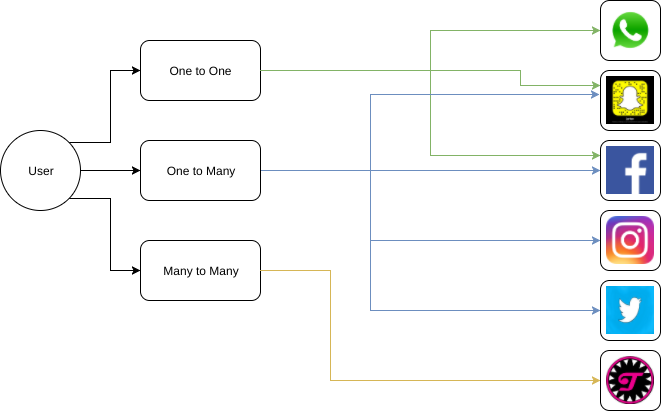
\includegraphics[scale=0.75]{similarServices}

	Talkatiel will be a Portable Web App, or a PWA.  This allows it to behave as an app does while also being much more accessible and easier to use for our end users.  The web app itself will consist primarily of 3 elements:   the service worker, the app shell, and the backend database.  A service worker is a chunk of code that exists outside the website.  It stays on a users device and works to cache and manage data for the web app.  It will also allow us to send push notifications to the user.  The app shell is the skeleton behind the web app.  It is stored on the users device, allowing the web app to load quickly.  It manages the basic user interface which is then filled with content from the server.  The database will store all posts along with identification and metadata information.

	Previously this idea has been attempted by Yik-Yak.  Originally released in 2013, Yik-Yak set out to solve many of the problems we are solving with Talkatiel.  One of the biggest issues that Yik-Yak encountered was bullying and harassment on the platform\cite{item1}.  The only moderation present in the app was an automod that deleted posts that had certain words.  This did not effectively deal with hurtful messages, only invited people to figure out better ways to circumvent the moderation.  To solve this, Talkatiel will use both word filtering and actual people to moderate.  As seen on sites like reddit, using trusted users to moderate other users can be a strong and effective tool.

	To build Talkatiel we will use Polymer for the user facing side.  It has been proven to be a simple and fast portable web app tool that allows us to quickly move from the idea stage to the testing stages of features.  Polymer is built on a mix of HTML, javascript, Node.js (4.x) and Bower.  The database will run on the google service FireBase.  This allows us to easily store and distribute user posts and settings and integrates easily with Polymer.  In addition to simply delivering data, Firebase also has extensive analytic and monitoring tools, allowing us to see the health of Talkatiel at a glance.

	We will be designing this for use primarily on mobile device browsers.  These include Chrome, Safari, and Firefox.  Because of the way PWA’s are structured, they should also perform well on desktop browsers such as Chrome, Edge, and Safari.

  Talkatiel will use a service worker to precache parts of a web app, allowing it to load quickly the next time the user uses it.  This allows us to manage what the user sees while cutting down on network traffic and load times.  A service worker can perform its tasks even when the web app isn’t open.  This means in addition to caching and managing web app data, it also has the ability to allow users to access things offline, intercept HTTP/HTTPS requests and even send push notifications to the user.
\subsection{Functional Requirements}
\subsubsection{Posting}
User will be able to create and post in discussions anonymously.  They will be able to read and respond to posts by other users.  Users will be able to reply to a discussion, reply to another reply and vote on posts.
\subsubsection{Moderation}
There will be both computer and real person moderation.  The computer run moderation will filter out posts will blacklisted words or phrases, while the human moderation will be done at the best judgment of whoever is moderating.
\subsubsection{Geolocation}
Users will only be able to post to certain discussions if they are with a range of the discussions marker.  If a user is within a certain distance they will be able to post to discussions.  If they are out of range of a discussion, they won’t be able to view or participate in the discussion.
\subsubsection{Viewing Posts}
Users will be able to scroll through posts made by others users.  They will be able to see the text of the post, and possibly how many votes the post has.  A user can then respond, vote, or continue scrolling to new content.
\subsubsection{Reporting}
Posts will be able to be reported for reason such as spam, abuse, bullying, or other issues.  These posts will then be dealt with by a human moderator, who can then choose to remove the post or let it be.  This will help cut out harmful speech that isn’t wanted on the platform.
\subsection{Non-Functional Requirements}
\subsubsection{Secure}
Talkatiel will need to utilize a secure connection (HTTPS).
All content needs to be delivered through a secure connection to confirm that all aspects of the app are controlled by us.  This tops malicious 3rd parties from abusing the service.
\subsubsection{Network Independent}
The app should still work when there is little or no network connectivity.
If not showing the different discussions, at least displaying a page notifying the user of the fact.  This will allow it to act as though it is a native app, though it is actually a website crafted for their device.  Also stops it from appearing "broken" to users, which could result in losing them.
\subsubsection{Responsive}
Talktatiel should be responsive to users on both phones and tablets.  The pwa should react quickly to user inputs, meaning that both the application presented to the user and the back-end database need to do their tasks speedily.
\subsubsection{Deep Linking}
Each page should have a distinct URL.  This means each discussion, post and reply should have it's own individual URL.  This allows user to share the post with others, such as on facebook or other social media services.
\subsubsection{Standard App Manifest}
Talkatiel should include a file that specifies all the metadata associated with it.
This allows us to set various settings for how the web app is displayed, such as orientation, display modes, image links, URL settings, and theming.  This is an integral part of making a portable web app and signals to browsers how to handle the website.
\subsection{Documentations}
In addition to a simple and intuitive user interface, there will also be a limited help section present.  It will show users how to do different basic functions of the application, such as navigating, posting, voting and the purpose.  The help section can walk a new user through the application and introduce them to the features.  By keeping the Talkatiel simple we can limit the amount of documentation needed while also improving user retention.
\subsection{Major Features}
\begin{itemize}
      \item Post text as part of discussion
      \item Reply to other user's posts
      \item Ability to vote up or down other posts
      \item Both computer and human moderation of posts
      \item Ability to participate and view discussions depending on location
      \item Ability to report posts to Moderators or Administrators
\end{itemize}
\subsection{Minor Feature / Strech Goals}
\begin{itemize}
      \item Ability to save discussions for later viewing.
      \item Ability for a user to view all of their own posts
      \item Keep track of the total votes a user has recieved
      \item Integrate ads into the platform
\end{itemize}

\section{Use Cases}

\subsection{Creating a new post}

\subsubsection{Goal}
User wants to create a new text or image post and publish it to the web app for others to see

\subsubsection{Actors}
College student users

\subsubsection{Preconditions}
The web app must first be loaded and the user must be on the create a new post page. The user must have GPS coordinates that are within the campus area

\subsubsection{Postconditions}
The web app will send the information to a firebase database of posts, which will update, displaying the new content on other users device

\subsubsection{Flow of Events}
\begin{itemize}
  \item user clicks create new post create post page is loaded from server
  \item user writes post and submits
  \item post text and title is pushed to posts table
  \item firebase post table is updated
  \item other users see updated post table when they load the posts page
\end{itemize}

\subsubsection{Quality Requirements}
The app content framework must load in less than a second, maximizing local caching to minimize external CDN requests.
The update request created by the posting of a new post must be processed in less than 5 seconds, and other users must be able to see the new post in less than 10 seconds


\subsubsection{Error Scenarios}
\textbf{Problem:}
 The user is not connected to the internet, post fails to publish
\textbf{Solution:}
  A page will load notifying the user that they have no connection to the internet
\textbf{Problem:}
  The database is down for maintenance or DDOS, user unable to post
\textbf{Solution:}
  A page will load notifying the user that posting is temporarily down, and to try again in a few minutes

\subsection{Auditing the new post}

  \subsubsection{Goal}
  Illegal posts won’t be able to post or they will be deleted later by administrators after receiving reports(break the anonymity rules: posts include personal phone number, email address ; contain illegal keywords: threatening or offensive language)


  \subsubsection{Actors}
  All users, administrator , word filter


  \subsubsection{Preconditions}
  Once users finish their posts and try to make a post, the word filter will be enabled. If the posts violate above rules, users will receive an alarm asks them to modify their post.


  \subsubsection{Postconditions}
   All posts will contain a report button in the bottom,  users are expected to maintain community stability by reporting illegal posts.


  \subsubsection{Flow of Events}
  \begin{itemize}
    \item user clicks post
    \item word filter is enabled and judge if the post legal
    \item post legal, update to server / post illegal,  asks user to modify the post
    \item  other user reviews the post
    \item  other users like the post / report the post
    \item administrator audits report post
    \item administrator adds the report post into word filter.
  \end{itemize}

  \subsubsection{Quality Requirements}
  All posts which get reported much be reviewed by administrator within 24 hr.
  Word filter must be updated monthly.


  \subsubsection{Error Scenarios}
  \textbf{Problem:}
  When illegal posts are prevented by word filter, but user doesn’t know what was wrong.
  \textbf{Solution:}
  highlight the illegal words.

\subsection{Viewing post page}

  \subsubsection{Goal}
  Users should be able to view all posts in a specified range ranked by a variety of chosen factors, (time posted, number of upvotes in different time range)
  \subsubsection{Actors}
  College student users

  \subsubsection{Preconditions}
  The web app must first be loaded and the user must be on the posts page. The user must be connected to the internet to load content.

  \subsubsection{Postconditions}
  The app must be able to connect to the posts database.

  \subsubsection{Flow of Events}
  \begin{itemize}
    \item User opens post page
    \item post page cached DOM framework loads
    \item web app queries server for posts with specific tags (time posted in range, topic)
    \item web app sorts posts by number of upvotes
    \item web app displays posts in DOM.

  \end{itemize}

  \subsubsection{Quality Requirements}
  Post page must load in less than 3 seconds
  Individual posts must load in less than 2 seconds


  \subsubsection{Error Scenarios}
  \textbf{Problem:}
  The user is not connected to the internet, post fails to publish
  \textbf{Solution:}
    A page will load notifying the user that they have no connection to the internet
  \textbf{Problem:}
  The database is down for maintenance / DDOS, user unable to view posts
  \textbf{Solution:}
    A page will load notifying the user that posting is temporarily down, and to try again in a few minutes

\section{Planning}
\subsection{Milestones}
\subsubsection{User Interaction}
	Users need to be able to easily read, comment, and make posts in real time. This is a challenge when there are fast updates and constant use. In addition to this, readers also need to be able to upvote and downvote posts, report posts, and save posts. Many of these features will need to be stored on a server, and most importantly, stored anonymously.
Location
	A user’s location will be general and only tied to their submitted posts and browsing. This data will only be stored when submitting a post.
\subsubsection{Backend Development}
	creating a strong and secure server will be challenging. Hosting a server will have more cons than pros, and renting a server may be safer for users. Getting the server setup will take a lot of time and effort to get it right. This means that a separate team will probably be assigned to 	develop this.
Server-side Storage
	Protecting user’s identity is very important. Things that are stored on a server like phone 	numbers and other identifiable information will be cached and stored on a local device. The 	only accounts that will exist are administrators (5 of us). These will be hashed and salted.
Risks
	Content such as posts and comments will be sent to the server. These will need to be checked for malicious code. This should happen quickly and reliably in order to have the user see the changes in a reasonable time. This will be tied to a unique user id, hidden on server side, in 	order to manage reports and bans.
Client-side Storage
	Users will have a cached version of the web-app, updating when refreshed or live feed. The app will have lightweight storage for the user.

\subsection{Timeline}
\subsubsection{HTML/CSS}
	02/12/18- This should be enough time to develop a clean, fully functioning look to the app. It needs to be mobile friendly as well.
\subsubsection{Javascript}
	02/19/18- Creating javascript is needed to make user interaction clean and send user data to the 	database. This should be secure and checked for vulnerabilities.
\subsubsection{Database}
	03/01/18- The database should be set up and functioning in 1 month from now. This means that 	the app will be functioning and ready for testing.
\subsubsection{Mobile Development}
	03/01/2018- This should be developed to work alongside the database and serve an identical 	copy of the website for PC. Mobile will be the main focus of this app, so it is crucial that it 	works well and is secure.

\subsection{Project Tracking}
\subsubsection{GitHub}
	We will be using GitHub to keep our code clean and organized. We have created a separate branch for these assignments and will be merging when complete. Github will allow us to store files neatly, and a seperate folder may be used for different teams.
\subsubsection{Slack}
	Slack has been very useful for many of us in the past. It allows us to communicate and stay on topic. We have everyone added and have been commenting and organizing meetings.
\subsubsection{Drive}
	A Google Drive folder has been created for our team. This allows us to manage files outside of github, such as photos, icons, useful links, notes, and written plans.

\subsection{Risk Management}
\subsubsection{Yik Yak}
	This idea was done by a company that has shutdown. Yik Yak made serious changes to their app in their final years, including trying to make a transition to a social media website. They added usernames, forced users to be accountable. We need to stay away from making the same mistakes, and make sure our users are hidden, otherwise we will fail.
\subsubsection{Storing User Data}
	Storing user data is very important. Users need to be able to trust our security before they use it. The best way to make sure the data is safe is to not collect much at all. This means that users will have very little to lose if our lack of experience with data protection results in a breach.
\subsubsection{Managing Content}
	Learning how to manage all of the content needed to make the website functioning could be difficult. Many different parts written by different people will need to be combined and work together flawlessly. THis means that we will need to communicate well and make sure that we are all on the same page.


\section{Meeting Report}

\subsection{Progress Made This Week}
	This week we completed the software requirements and planning phase of the project.  We worked on defining both functional and non-functional requirements along with use cases.  Finally, we created a project plan that outlines the different phases of the project, including backend development, frontend development, user interface, user experience, and potential issues.  We will continue to communicate on Slack to coordinate another meeting time.
\subsection{Plans for Next Week}
	In the coming week we will start mapping out the architecture of the pwa.  Work will start with planning out the different views in the application.  Along with this we will start looking at how we should store the data, e.g. data structures and such.  Team members are going to start experimenting and getting comfortable with both Polymer and Firebase so once we get into the coding portion everything won’t be new.  Along with this we are going to work on the requirements more and get a plan for each one, detailing what needs to go into each one.
\subsection{Team Member Contributions}
	Brendan Byers worked on the description and bibliography section.
	Aiden Grimshaw worked use cases, table of contents, and latex formatting.
	Ryan Sisco worked on the planning section
	Yufei Zeng worked on use cases and latex formatting

\subsection{Customer Meeting Status}
	We met with the customer and worked on getting general requirements set.  We talked about what the end goal should look like, along with optional goals that we may want to work on if we have time at the end.  The customer is very happy with how things are coming along.

\newpage
  \begin{thebibliography}{1}

  \bibitem{item1} Lindsay Bramson {\em Yik Tak bullying leads district to ban app}  2014: KXAN.com. http://kxan.com/2014/09/29/yik-yak-bullying-leads-districts-to-ban-app/

  \bibitem{item2}  Nick Strayer {\em The Great Out-Of-State Migration: Where Students Go} 2016:
  New York Times. https://www.nytimes.com/interactive/2016/08/26/us/college-student-migration.html

  \end{thebibliography}

\end{document}
